\subsection{Scalability - SCVM Vectorization}
\label{sec:Method:Scalability}
A key focus of this project was to make the model scalable, in order to enable the modelling of larger, more realistic networks.
This subsection therefore describes vectorization of the model which was the essential foundation for utilizing the GPU parallelization capabilities of Pytorch CUDA\cite{CUDADocumentation} in order to dramatically improve the code execution time.

\subsubsection{Vectorized Latent Space Position Calculation}
\label{sec:Method:LatentSpacePositionCalculation}
To compute the node latent space positions in a vectorized manner, it is necessary to change the computation from working on specific pair of nodes to working directly on $\textbf{Z}$ and $\textbf{V}$. Since $\textbf{V}$ is a tensor of shape $\mathbb{R}^{N \times 2 \times S}$, $N$ and $S$ being the number of nodes and steps respectively, we have to also adjust the $\Delta_j(t)$ representation from (\ref{eq:delta_t}), such that it becomes a vector representation of the portions of the time point $t$ that falls into each time step bin of the $S$ dimension in $\textbf{V}$.
\\
For this the model uses a $step$ function which takes as input a vector $\textbf{t} \in \mathbb{R}^{T}$ of $T$  time points from the node pair interaction data. Each time point $t$ in $\textbf{t}$ is then binned into a vector $\boldsymbol{\Delta}\textbf{t} \in \mathbb{R}^{S}$ where $\boldsymbol{\Delta}\textbf{t}_j \in \mathbb{R}$ is the portion $\Delta t$ of $t$ that falls into the $j$'th step of the velocities. From all these $\boldsymbol{\Delta}\textbf{t}$ vectors a matrix $\boldsymbol{\Delta}\textbf{T} \in \mathbb{R}^{T \times S}$ is created such that:
\begin{align}
    \boldsymbol{\Delta}\textbf{T}_{i,\;j} =
    \begin{cases}
        \Delta_{step} \;\; &\text{for} \;\; t_i >= (\Delta_{step} \cdot j) \\
        \text{max}(0, t_i + \Delta_{step} - \Delta_{step} \cdot j) \;\; \;\; &\text{for} \;\; t_i < (\Delta_{step} \cdot j)
    \end{cases}
    \;\; \forall \;\; t_i \in \textbf{t}
\end{align}
Where $j \in \{1,2,...,S\}$ is the step index. A visual example of this is shown below:
\begin{figure}[H]
    \centering
    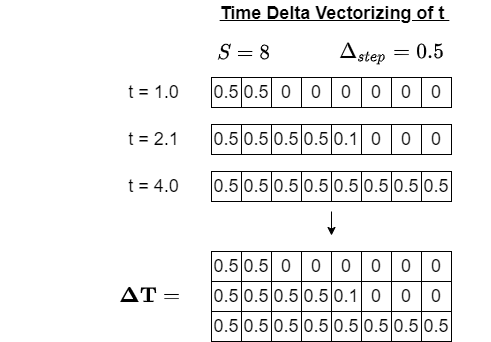
\includegraphics[width=0.5\textwidth]{0_images/time_deltas.png}
    \caption{Example of splitting $\textbf{t} \in \mathbb{R}^3$ time points into time delta matrix $\boldsymbol{\Delta}\textbf{T} \in \mathbb{R}^{3 \times 8}$}
    \label{Method:Vectorized:fig:time_delta_split}
\end{figure}
\\
\noindent
It is now possible to calculate the node movements for every node to every time in \textbf{t} by first computing the product of $\boldsymbol{\Delta}\textbf{T}$ broadcasted\cite{BroadcastingDocumentation} onto $\textbf{V}$ by unsqueezing the $S$ dimension of $\textbf{V}$, such that $\mathbb{R}^{N \times 2 \times S} \rightarrow \mathbb{R}^{N \times 2 \times 1 \times S}$. The product will then create a tensor of size $\mathbb{R}^{N \times 2 \times T \times S}$ and by summing over the $S$ dimension we then get the node movements for the time points in $T$ as a 3-dimensional tensor $\boldsymbol{\mathcal{M}} \in \mathbb{R}^{N \times 2 \times T}$.
\lstinputlisting[language=Python]{code_snippets/movement.py}
\\
The latent space node positions $\textbf{Z}_{t}$ for all nodes at all times in $\textbf{t}$ can then be calculated as the latent starting positions at time 0, $\textbf{Z}$ broadcasted over the time dimension in the movements i.e. unsqueezing $\textbf{Z}$ so its shape changes $\mathbb{R}^{N \times 2 \times 1}$ and then summing with $\boldsymbol{\mathcal{M}}$:
\lstinputlisting[language=Python]{code_snippets/latent_pos.py}
\\
When this process is applied we get a collection of latent position matrices $\textbf{Z}_t$ according to the number of time points in $\textbf{t}$ i.e. $\textbf{Z}_t \in \mathbb{R}^{N\text{x}D\text{x}T}$, which can be used to compute the event intensity for each node pair interacting at each time point.

\paragraph{Vectorized Loss Function}
Now calculating the event intensity first becomes a matter of computing the node pairwise squared Euclidean distance matrix for all time points $\boldsymbol{\mathcal{D}}_t$ i.e. the squared Euclidean distances for each time in $\textbf{Z}_t$. This can be done by broadcasting $\textbf{Z}_t$'s node dimension $N$ onto its latent space dimension $D=2$.
\lstinputlisting[language=Python]{code_snippets/temporal_dist.py}
\\
This will produce the node temporal pairwise squared Euclidean distance matrix $\boldsymbol{\mathcal{D}}_t^{N \times N \times T}$.
Where \texttt{Z.unsqueeze(0)-Z.unsqueeze(1)} is the broadcasting, which produces a tensor with shape $\mathbb{R}^{N \times N \times 2 \times T}$, that holds the $x$- and $y$-coordinate differences between the node pairs for all the time points. 
The log intensity tensor then becomes the subtraction of the common bias and $\boldsymbol{\mathcal{D}}_t$:
\begin{equation}
    \boldsymbol{\mathcal{I}}_e = \beta \cdot \textbf{1} - \boldsymbol{\mathcal{D}}_t
\end{equation}
Where $\textbf{1}$ is a tensor of ones with the same shape as $\boldsymbol{\mathcal{D}}_t$ used to broadcast $\beta$ which is done "under the hood" by Pytorch. Then from $\boldsymbol{\mathcal{I}}_e$ we can now select and sum the log intensities for each node pair at their given interaction time by slicing the tensor:
\lstinputlisting[language=Python]{code_snippets/vec_event_intensity.py}
\\
The non-event intensity can be computed in much the same way as in equation (\ref{eq:analytical_integral}), by having $a, b, m$, and $n$ be vectorized to contain the subtration of all $x$ and $y$ coordinates for the starting positions and the velocities for each step in the model. This will result in the tensors $\textbf{a}, \textbf{b} \in \mathbb{R}^{N \times N \times S}$ which are the node pairwise differences in the node latent position coordinates $x$ and $y$ for each step. $\textbf{m}, \textbf{n} \in \mathbb{R}^{N \times N \times S}$ are then the node pairwise differences in the node velocity coordinates $x$ and $y$ for each step. This again can be implemented in Pytorch through broadcasting: 

\lstinputlisting[language=Python]{code_snippets/analytical_integral.py}
\\
Where \texttt{torch.eps} is added to make sure the integral does end up being undefined.
\\
The analytical integral function will now produce a tensor with shape $\mathbb{R}^{N \times N \times S}$ which contains the pairwise node interaction intensities for each step. The non-event intensity $I_n$ can then be computed as the upper triangular sum of the intensities over the steps. In Pytorch this vectorized computation can be done as:

\lstinputlisting[language=Python]{code_snippets/non_event_vectorized.py}
\noindent
Then the loss can again be computed as $\mathcal{L} = - I_e - I_n$. Here the regularization from (\ref{eq:Method:ProposedModel:vec_regularization}) can also be applied directly, as it is already vectorized.